% !TeX spellcheck = de_CH
\documentclass[
a4paper,
oneside,
landscape, 
8pt,
]{scrartcl}

% language
\usepackage[T1]{fontenc}
\usepackage[utf8]{inputenc}

% tables
\usepackage{tabu}
\usepackage{booktabs}
\tabulinesep=1.2mm

% images
\usepackage{graphicx}

% layout
\usepackage[landscape]{geometry}
\geometry{tmargin=5mm,bmargin=5mm,lmargin=5mm,rmargin=5mm}
\usepackage{multicol}
\setlength{\columnsep}{1cm}

% math
\usepackage{amsmath}
\usepackage{amssymb}
\usepackage{amsfonts}
\usepackage{enumitem}
 
% title
\title{PhAI: Physik Anwendungen für Informatiker}
\subject{Cheatsheet}
\author{Michael Wieland}
\date{\today}


\begin{document}

\maketitle



\begin{multicols*}{2}
	
\tableofcontents
\clearpage
	
\section{Grundlagen}
\subsection{Konstanten}
\begin{tabbing}
	\begin{tabu} to \linewidth {l X l }
		\toprule
		Konstante & Bedeutung & Wert \\
		\midrule
		$u$ & Atomare Massenkonstante & $1.660538921(73) \cdot 10^{-27} kg$\\
		$N_A$ & Avogadro Konstante = 1mol & $6.022141 29 (27) \cdot 10^{23} \frac{1}{mol}$  \\
		$k_b$ & Boltzmann-Konstante & $1.3806488(13) \cdot 10^{-23}\frac{J}{K}$  \\
		$R$ & Universelle Gaskonstante & $N_A \cdot k_B = 8.3144621 (75) \frac{J}{mol \cdot K}$ \\
		$g$ & Normalfallbeschleunigung(Schwerkraft auf der Erde) & $9.80665\frac{m}{s^2}$ \\
		$T_n$ & Normtemperatur & $273.15K$  \\
		$\sigma$ & Stefan-Boltzmann-Konstante & $5.670373(21) \cdot 10^{-8} \frac{W}{(m^2 \cdot K^4)}$  \\
		$c$ & Lichtgeschwindigkeit & $3 \cdot 10^8 \frac{m}{s}$  \\
	\end{tabu}
\end{tabbing}

\subsection{Umrechnungen}
Physikalische Dimension: Masse, Länge, Zeit, Temperatur, Stromstärke, Lichtstärke, Stoffmenge.
\begin{tabbing}
	\begin{tabu} to \linewidth {l X}
		\toprule
		Volumen & $1cm^3 = (10^{-2}m)^3 = 10^{-6}m^3$ \\ 
		Fläche &  $1cm^2 = (10^{-2}m)^2 = 10^{-4}m^2$ \\
		Geschwindigkeit & $1\frac{m}{s} = 3.6\frac{km}{h} = 1\frac{km}{h} = 0.277 \frac{m}{s}$ \\
		Grad in Fahrenheit & $T_F = \frac{9}{5} \cdot T_C + 32 \Rightarrow 0^\circ\text{C} = 32F$ \text{und} $100^\circ\text{C} = 212F$ \\ 
		Grad in Kelvin & $T_K = T_C + 273.15$ \\
		Bar in Pascal & $1 bar = 100'000 \frac{N}{m^2} = 100'000 Pa (=10^5)$ \\
		kWh in kJ & $1kWh = 1000W \cdot 3600 s= 3.6 \cdot 10^6 Ws = 3.6 MJ = 3600kJ = 3.6 \cdot 10^6 J$ \\
		kcal in Joule & $1kcal = 4184 J$ \\
		Watt in PS & $1KW = 1.36PS$ und $1PS = 735.499W$ \\
		Bogenmass (rad) in Gradmass & $2\pi \mathrm{rad} = 360^\circ $\\
		Steigung in Prozent/Grad & $\text{Steigungswinkel}(^\circ) = arctan( Steigung(\%) / 100 )$ \\	
		\bottomrule
	\end{tabu}
\end{tabbing}

\subsection{Planimetrie und Stereometrie}

\begin{tabbing}
	\begin{tabu} to \linewidth {l l X l X}
		\toprule
		\textbf{Trapez} & Fläche & $A = \frac{a + c}{2} \cdot h$ & 
		Umfang & $U = 2 \cdot h  + a + c$ \\
	\end{tabu}
\end{tabbing}

\begin{tabbing}
	\begin{tabu} to \linewidth {l l X l X}
		\textbf{Dreieck} & Fläche & $A = \frac{g \cdot h}{2}$ & 
		Sinus & $\sin(\alpha) = \frac{G}{H}$ \\
		& Cosinus & $\cos(\alpha) = \frac{A}{H}$ &
		Tangens &  $\tan(\alpha) = \frac{G}{A}$ \\
	\end{tabu}
\end{tabbing}


\begin{tabbing}
	\begin{tabu} to \linewidth {l l X l X}
		\textbf{Kreis} & Fläche & $A = r^2 \cdot \pi$ & 
		Umfang & $U = 2 \cdot r \cdot \pi$ \\
	\end{tabu}
\end{tabbing}


\begin{tabbing}
	\begin{tabu} to \linewidth {l l X l X}
		\textbf{Kreis} &  Fläche & $A = \frac{d^2 \cdot \pi}{4}$ &
		Volumen & $V = r^2 \cdot \pi \cdot h $ \\
		& Mantelfläche & $M = d \cdot \pi \cdot h$ &
		Oberfläche & $O = M + 2 \cdot A $ \\
		\bottomrule
	\end{tabu}
\end{tabbing}

\paragraph{Kegel}
\begin{tabbing}
	\begin{tabu} to \linewidth {l X l X}
		\toprule
		Fläche & $A = \frac{3 \cdot V}{h}$ &
		Volumen & $V = \frac{A \cdot h}{3}$ \\
		Höhe & $h = \frac{3 \cdot V}{A}$ & & \\
		\bottomrule
	\end{tabu}
\end{tabbing}

\subsection{Vektoren}

\begin{itemize}
	\item Beim Vektorprodukt entsteht ein neuer Vektor, der senkrecht auf den beiden Ausgangsvektoren steht, wenn diese linear unabhängig sind.
	\begin{itemize}
		\item Spannen die beiden Ausgangsvektoren ein Parallelogramm auf, so ist der Betrag des Vektorprodukts gleich dem Flächeninhalt des Parallelogramms.
	\end{itemize}
	\item Das Skalarprodukt zweier Vektoren ist null, wenn sie senkrecht zueinander stehen.
	\item Die Multiplikation zweier Vektoren (Skalarprodukt) ergibt eine reelle Zahl (Skalar)
\end{itemize}

\begin{tabbing}
	\begin{tabu} to \linewidth {l X}
		\toprule
		Vektorprodutk / Kreuzprodukt & $
		\vec{a}\times\vec{b}
		=
		\begin{pmatrix}a_x \\ a_y \\ a_z\end{pmatrix}
		\times
		\begin{pmatrix}b_x \\ b_y \\ b_z \end{pmatrix}
		=
		\begin{pmatrix}
		a_yb_z - a_zb_y \\
		a_zb_x - a_xb_z \\
		a_xb_y - a_yb_x
		\end{pmatrix}\,.
		$ \\
		Eingeschlossener Winkel & $\sin(\alpha) = \frac{|\vec{a}|\, |\vec{b}|}{|\vec{a}\times\vec{b}|}$\\
		Skalarprodukt & $\vec a \cdot \vec b = a_x b_x + a_y  b_y +  a_z  b_z$ \\
		Länge eines Vektors (Betrag) & $| \vec a | = \sqrt{\vec a\cdot \vec a} = \sqrt{{a_x}^2+{a_y}^2+{a_z}^2}$ \\
		Eingeschlossener Winkel & $\cos (\alpha) = \frac{\vec a\cdot\vec b}{|\vec a|\,|\vec b|}$ \\
		\bottomrule
	\end{tabu}
\end{tabbing}


\subsection{SI-Einheiten}
\begin{tabbing}
	\begin{tabu} to \linewidth {l l X}
		\toprule
		Einheit & Zeichen & Einheit für \\
		\midrule
		Ampere  & A & elektr. Stromstärke \\
		Coulomb & cd & elektr. Ladung \\
		Grad Celsius & $^\circ C$ & Temperatur \\
		Hertz & Hz & Frequenz \\
		Joule & $J = N \cdot m = W \cdot s$ & Energie, Arbeit, Wärmemenge \\
		Kelvin & K & absolute Temperatur \\
		Kilogramm & kg & Masse \\
		Meter & m & Länge \\
		Mol & mol & Stoffmenge \\
		Newton & $N = \frac{kg}{m/s^2}$ & Kraft \\
		Ohm & $\Omega = \frac{V}{A}$ & elektr. Widerstand \\
		Pascal & $Pa = \frac{N}{m^2}$ & Druck, Spannung \\
		Sekunde & s & Zeit\\
		Volt & $V = \frac{W}{A}$ & elektr. Spannung\\
		Watt & $W = \frac{J}{s}$ & Leistung \\
		\bottomrule
	 \end{tabu}
\end{tabbing}



\vfill\null
\columnbreak


\section{Mechanik}

\subsection{Statik}

\subsubsection{Drehmoment}

\begin{itemize}
	\item Die wirksame Hebellänge wird begrenzt zwischen dem Drehpunkt und dem Ansatzpunkt der Kraft
	\item Mehrere Drehmomente im Gegenuhrzeigersinn (positives Vorzeichen) und im Uhrzeigersinn (Vorzeichen) sind im Gleichgewicht, wenn das Gesamtdrehmoment $M_{tot}$ null ist.
	\item \textbf{Hebelgesetz}: Kraft $\cdot$ Kraftarm = Last $\cdot$ Lastarm
	\item Der Bezugspunkt P ist frei wählbar
	\item Das Drehmoment ($M = J \alpha$) ist für die Rotation, die Kraft in der Translation ($F = ma$)
\end{itemize}

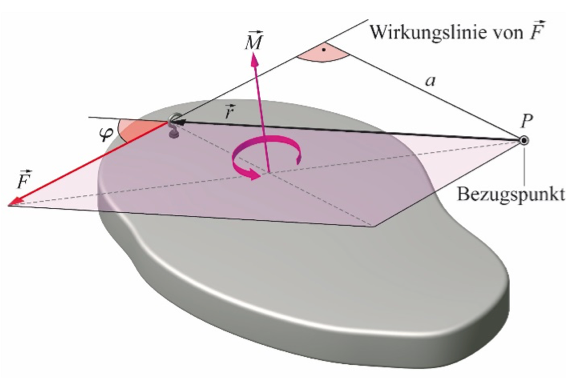
\includegraphics[width=0.4\linewidth]{images/drehmoment}

\begin{tabbing}
	\begin{tabu} to \linewidth {l X l X}
		\toprule
		Hebelgesetz & $F_1l_1 = F_2l_2 \Leftrightarrow M_1 = M_2$ & 
		Drehmoment & $M = F \cdot r \cdot \sin(\varphi)$ \\
		Drehmoment & $M = J \cdot \alpha$ & 
		Trägheitsmoment & $J = m r^2$ \\
	\end{tabu}
\end{tabbing}

\begin{tabbing}
	\begin{tabu} to \linewidth {l X l}
		Variable & Bedeutung & SI-Einheit \\
		\midrule
		$M$ & Drehmoment & $Nm$ \\ 
		$F$ & wirkende Kraft & $Nm$ \\ 
		$r$ & Abstand Bezugspunkt-Angriffspunkt & $m$ \\ 
		$a$ & Hebelarm: senkrechter Abstand Bezugspunkt-Wirkungslinie der Kraft & $m$ \\ 
		$P$ & Bezugspunkt: Frei wählbar & \\
		\bottomrule
	\end{tabu}
\end{tabbing}


\begin{minipage}[h!]{0.5\linewidth}
	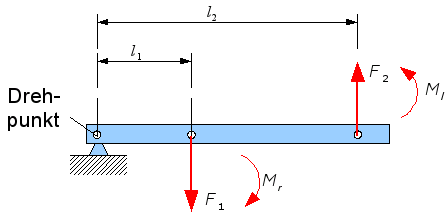
\includegraphics[width=0.8\linewidth]{images/hebel_einseitig}
\end{minipage}
\hfill
\begin{minipage}[h!]{0.5\linewidth}
	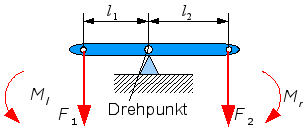
\includegraphics[width=0.8\linewidth]{images/hebel_zweiseitig}
\end{minipage}



\begin{minipage}[h!]{0.5\linewidth}
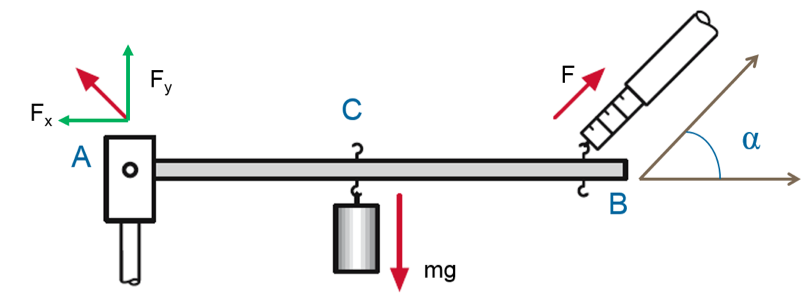
\includegraphics[width=0.9\linewidth]{images/hebel}
\end{minipage}
\hfill
\begin{minipage}[h!]{0.5\linewidth}
	
	\begin{align*}
	M_A &:	F  \cdot r \cdot  \sin(\alpha) - m g \cdot \frac{r}{2} = 0 \\
	\Rightarrow F &= \frac{mg}{2 \sin(\alpha)} \\
	X&:	F \cos(\alpha) - F_x = 0 \\ 
	Y&:	F \sin(\alpha) + F_y - m g = 0 \\ 
	\Rightarrow F_x &= F \cos(\alpha) \text{ und } F_y = mg - F \sin(\alpha) \\
	\Rightarrow F_{t} &= F_1 + F_2 \\
	\end{align*}
	
\end{minipage}


\vfill\null
\columnbreak



\subsubsection{Gleichgewicht}
\begin{itemize}
	\item Ein Massenpunkt ist im Gleichgewicht wenn die Summe der Kräfte gleich null ist. 
\end{itemize}

\begin{tabbing}
	\begin{tabu} to \linewidth {l X}
		\toprule
		Kräftegleichgewicht & 
		$\vec{F}_{res} = \vec{F}_1 +\vec{F}_2 + .. + \vec{F}_n \Rightarrow  \sum_{i=1}^{n}\vec{F}_i = \vec{0}
		\Rightarrow  \sum_{i=1}^{n}\vec{M}_i = \vec{0}$ \\
		Massenmittelpunkt & $\sum_{i=1}^{n} \frac{r_i \cdot m_i}{m_ges}$ \\
		\bottomrule
	\end{tabu}
\end{tabbing}

\begin{tabbing}
	\begin{tabu} to \linewidth {l X l}
		Variable & Bedeutung & SI-Einheit \\
		\midrule
		$m_i$ & Massenelemente &  \\ 
		$r_i$ & Ortsvektoren der Massenelemente &  \\ 
		\bottomrule
	\end{tabu}
\end{tabbing}

Die Summe muss mit Vektoraddition ausgerechnet werden. Nach Festlegung eines Koordinatensystems kann mit Komponenten der Vektoren gerechnet werden. In zwei Dimensionen erhalten wir somit zwei Gleichungen und können maximal zwei Unbekannte bestimmen.


\begin{minipage}[h!]{0.5\linewidth}
	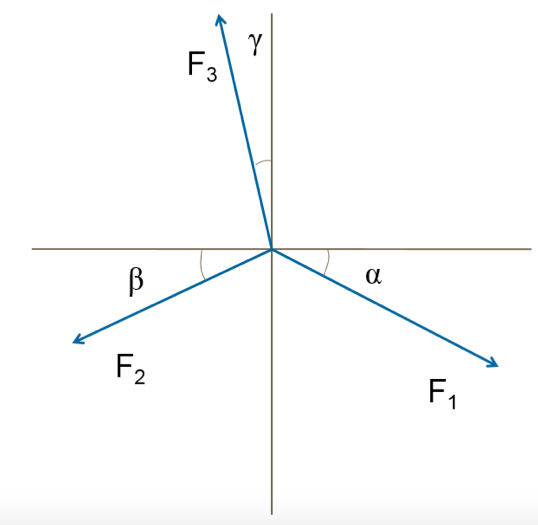
\includegraphics[width=0.7\linewidth]{images/gleichgewicht}
\end{minipage}
\hfill
\begin{minipage}[h!]{0.5\linewidth}
	
	\begin{align*}
	X &: F_1  \cos(\alpha) - F_2  cos(\beta) - F_3 \sin(\gamma) = 0 \\
	Y &: -F_1  \sin(\alpha) - F_2 \sin(\beta) + F_3 \cos(\gamma) = 0
	\end{align*}
	
\end{minipage}

\subsubsection{Schwerpunkt}
Die Gewichtskraft eines Körpers ist gleich der Summe der Gewichtskräfte seiner Teilchen. Die Summe der Gewichtskräfte greift im Schwerpunkt an. 
\begin{itemize}
	\item Wenn ein Körper im Schwerpunkt aufgehängt wird, ist er im Gleichgewicht. Somit ist das Drehmoment um den Schwerpunkt = 0
	\item Die Schwerkraft, welche auf einen starren Körper wirkt, kann durch eine Kraft im Schwerpunkt ersetzt werden. $r_p \sum_{i} m_i = \sum_{i} m_i  r_i$
\end{itemize}


\vfill\null
\columnbreak


\subsection{Kinematik}
\begin{itemize}
	\item Man unterscheidet zwei Arten von Bewegungen
	\begin{itemize}
		\item Translation (geradlinige Bewegung)
		\item Rotation (Drehbewegung)
	\end{itemize}
	\item Die meisten Kinematikaufgaben können am einfachsten mit einem v-t Diagramm gelöst werden. Die Fläche unter der Kurve stellt die Geschwindigkeit dar. Die Steigung der Kurve ist die Beschleunigung.
\end{itemize}


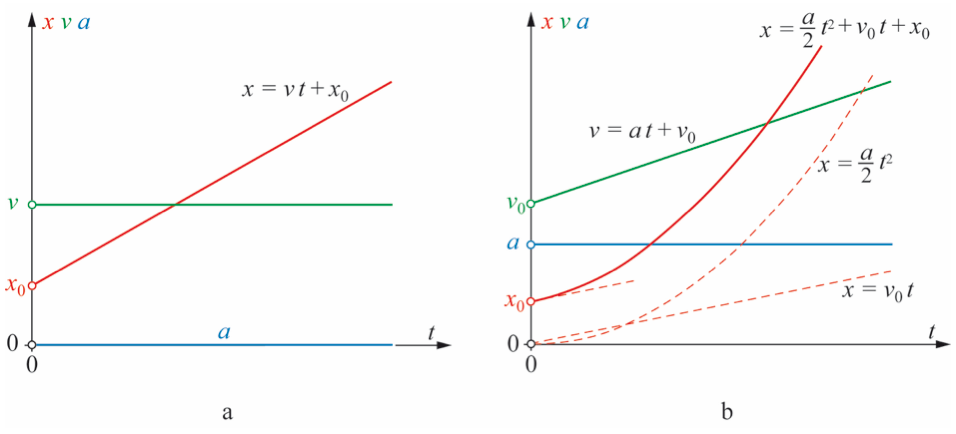
\includegraphics[width=0.7\linewidth]{images/kinematik}

\subsubsection{Translation}
\begin{tabbing}
	\begin{tabu} to \linewidth {X l l}
		\toprule
		Art & Geschwindigkeit v & Beschleunigung a \\
		\midrule
		gleichförmig & konstant & 0 \\
		gleichmässig beschleunigt & ändert sicht gleichmässig & konstant \\
		ungleichmässig beschleunigt & ändert sich ungleichmässig & ändert sich \\
	\end{tabu}
\end{tabbing}


\paragraph{Konstante Geschwindigkeit (gleichförmig)}

\begin{tabbing}
	\begin{tabu} to \linewidth {l X l X l X}
		\toprule
		Geschwindigkeit & $v = \frac{s}{t}$ &
		Strecke & $s = v \cdot t + s_0$ &
		Zeit & $t = \frac{s}{v}$ \\
		\bottomrule
	\end{tabu}
\end{tabbing}

\paragraph{Konstante Beschleunigung (gleichmässig)}

\begin{tabbing}
	\begin{tabu} to \linewidth {l X X}
		\toprule
		& Ohne Anfangsgeschwindigkeit & Mit Anfangsgeschwindigkeit \\
		\midrule
		Beschleunigung & 
		$a = \frac{\Delta v}{ \Delta t} = \dfrac{v^2}{2s} = \dfrac{2s}{t^2}$ &
		$a = \frac{v^2 - v_0^2}{2s}$ \\
		Geschwindigkeit & 
		$v = a \cdot t = \sqrt{2 a s}$ &
		$v = \sqrt{2a(s-s_0) + v_0^2} = a \cdot t + v_0 $ \\
		$\varnothing$ Geschwindigkeit & 
		$v_m = \frac{v_1 + v_2}{2} = \frac{at}{2} = \frac{s}{t}$ &
		 \\
		Strecke & 
		$s = \frac{v t}{2} = \frac{a t^2}{2} = \frac{v^2}{2a}$ &
		$s = \frac{1}{2} at^2 + v_0 t + s_0 = \frac{v^2 - v_0^2}{2a} $ \\
		Zeit & 
		$t = \frac{v}{a} = \sqrt{\frac{2s}{a}}$ & \\		
	\end{tabu}
\end{tabbing}

\begin{tabbing}
	\begin{tabu} to \linewidth {l X l}
		Variable & Bedeutung & SI-Einheit \\
		\midrule
		$v$ & Geschwindigkeit  & $\frac{m}{s}$ \\ 
		$a$ & Beschleunigung  & $\frac{m}{s^2}$ \\ 
		$t$ & Zeit  & $s$ \\ 
		$s$ & Strecke  & $m$ \\ 
		\bottomrule
	\end{tabu}
\end{tabbing}

\subsubsection{Rotation}

\begin{itemize}
	\item Eine Rotation heisst gleichförmig, wenn die Winkelgeschwindigkeit $\omega$ konstant ist. 
	\item Die Tangentialgeschwindigkeit ($\vec{v}=\omega r$) ist die Geschwindigkeit die in der Rotation gerade aus geht
\end{itemize}

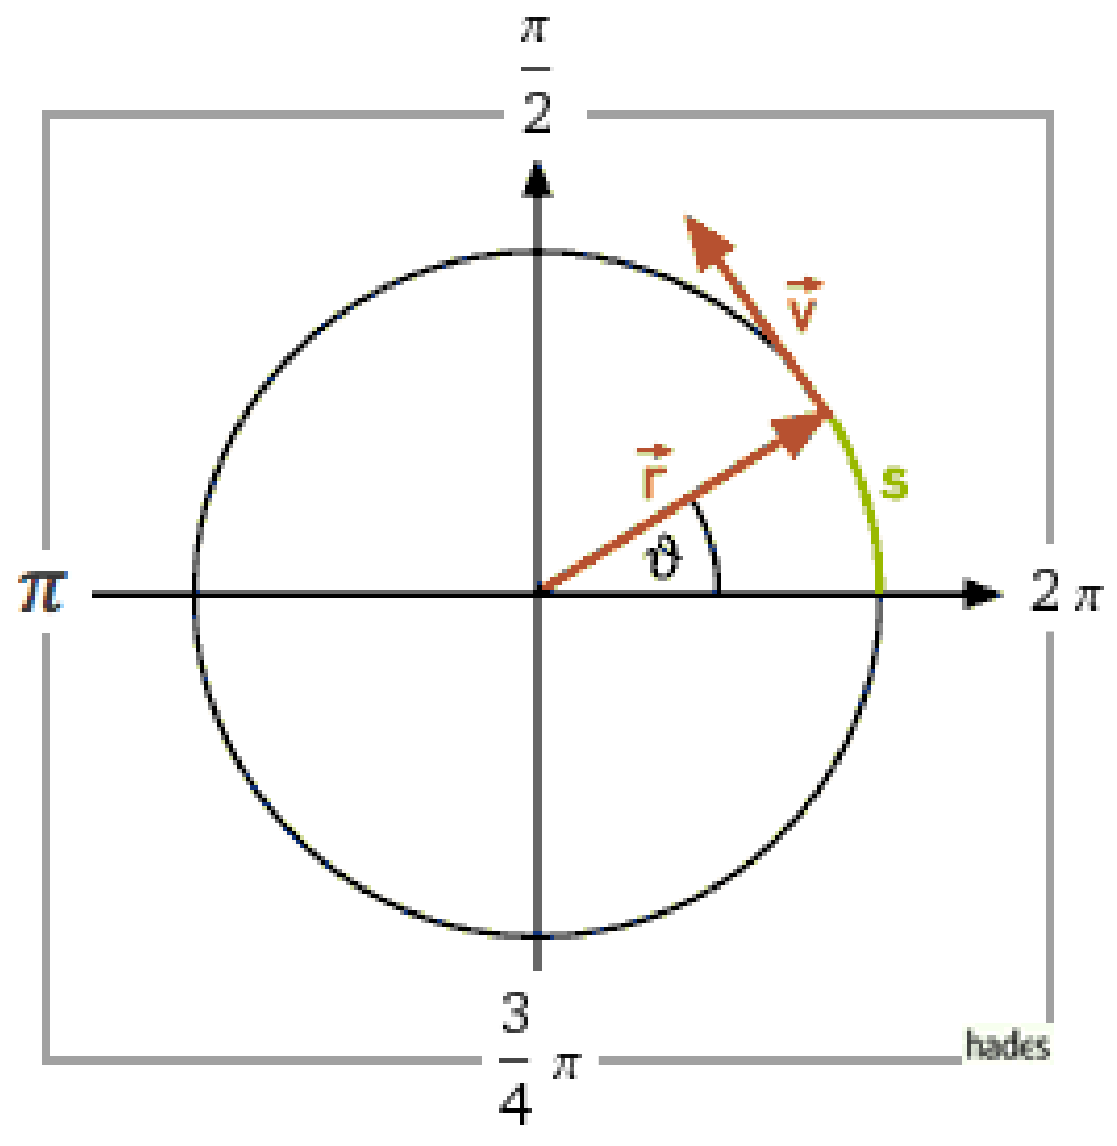
\includegraphics[width=0.2\linewidth]{images/rotation}

\paragraph{Konstante Geschwindigkeit (gleichförmig)}

\begin{tabbing}
	\begin{tabu} to \linewidth {l X l X}
		\toprule
		Winkelgeschwindigkeit & $\omega = \frac{\varphi}{t} = 2 \pi f$ &
		Rotationswinkel & $\varphi = \omega \cdot t$ \\
		Zeit & $t = \frac{\varphi}{\omega}$ &
		Drehzahl & $n = \frac{z}{t} = \frac{1}{T} = \frac{\omega}{2 \pi}$  \\
		Periodendauer & $T = \frac{1}{n} = \frac{2\pi r}{v} = \frac{2\pi}{\omega}$ &
		Anz. Umdrehungen & $N = \frac{\varphi}{2 \pi}$ \\
		\bottomrule
	\end{tabu}
\end{tabbing}

\paragraph{Konstante Beschleunigung (gleichmässig)}

\begin{tabbing}
	\begin{tabu} to \linewidth {l X X}
		\toprule
		& Ohne Anfangsgeschwindigkeit & Mit Anfangsgeschwindigkeit \\
		\midrule
		Winkelbeschleunigung & 
		$\alpha = \frac{\omega}{t} = \frac{2 \varphi}{t^2} = \frac{\omega^2}{2 \varphi}$ &
		$\alpha = \frac{\omega^2 - \omega_0^2}{2 \varphi}$ \\
		Winkelgeschwindigkeit & 
		$\omega = \alpha t = \sqrt{2 \alpha \varphi}$ &
		$\omega = \alpha t + \omega_0 = \sqrt{2\alpha \varphi + \omega_0^2} $ \\
		$\varnothing$ Winkelgeschwindigkeit & 
		$\omega_m = \frac{\alpha t}{2} = \frac{\varphi}{t}$ & \\
		Rotationswinkel & 
		$\varphi = \frac{\omega t}{2} = \frac{\omega^2}{2 \alpha} = \frac{\alpha t^2}{2} = \frac{s}{r} = 2\pi N$ &
		$\varphi = \frac{(\omega_0 + \omega_1)t}{2} = \frac{\omega^2 - \omega_0^2}{2 \alpha} = \frac{\alpha t^2}{2} + \omega_0 t + \varphi_0$ \\
	\end{tabu}
\end{tabbing}

\paragraph{Umrechnung Translation und Rotation}

\begin{tabbing}
	\begin{tabu} to \linewidth {l X l X l X}
		\toprule
		Geschwindigkeit & $v = r \cdot \omega$ &
		Beschleunigung & $a = r \cdot \alpha$ &
		Strecke & $s = r \cdot \varphi$ \\
		Winkelgeschwindigkeit & $\omega = \frac{v}{r}$ &
		Winkelbeschleunigung & $\alpha = \frac{a}{r}$ &
		Rotationswinkel & $\varphi = \frac{s}{r}$ \\
		\bottomrule
	\end{tabu}
\end{tabbing}

\begin{tabbing}
	\begin{tabu} to \linewidth {l X l}
		Variable & Bedeutung & SI-Einheit \\
		\midrule
		$\varphi$ & Rotationswinkels  & rad (Bogenmass) \\ 
		$\omega$ & Winkelgeschwindigkeit & $\frac{rad}{s}$ \\
		$\alpha$ & Winkelbeschleunigung & $\frac{rad}{s^2}$ \\
		$n = f$ & Drehzahl rsp. Umdrehungsfrequenz & $\frac{1}{s} = Hz$ \\
		$N$ & Anzahl ausgeführte Umdrehungen & \\
		$T$ & Periodendauer, Umlaufdauer & $s$ \\
		$t$ & Zeit die für die Drehung um den Winkel $\varphi$ benötigt wird & $s$ \\
		$s$ & Weg beim Umfang & $m$ \\
		$r$ & Radius & $m$ \\
		$z$ & Anzahl der Umdrehungen während der Zeit t & \\
		\bottomrule
	\end{tabu}
\end{tabbing}


\clearpage


\subsubsection{Fall und Wurf}

\paragraph{Freier Fall}
\begin{itemize}
	\item Beim freien Fall wird eine gleichmässig beschleunigte Bewegung durch die Erdanziehung hervorgerufen. ($a = g$ und $s = h$)
\end{itemize}
\begin{tabbing}
	\begin{tabu} to \linewidth {l X l X}
		\toprule
		Höhe & $h = \frac{vt}{2} = \frac{gt^2}{2}$  &
		Geschwindigkeit & $v = gt = \sqrt{2gh}$ \\
		Zeit & $t = \sqrt{\frac{2h}{g}}$ & & \\
		\bottomrule
	\end{tabu}
\end{tabbing}


\paragraph{Schiefer Wurf}

\begin{itemize}
	\item $45^\circ$ ist der optimale Winkel, falls keine Höhe überwunden werden muss!
\end{itemize}

\begin{minipage}[h!]{0.6\linewidth}
	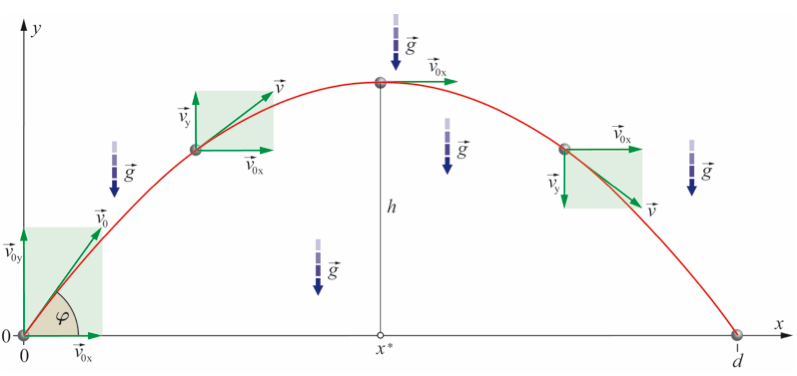
\includegraphics[width=0.9\linewidth]{images/schiefer_wurf}
\end{minipage}
\hfill
\begin{minipage}[h!]{0.4\linewidth}
Bahngleichung des Schiefen Wurfs: 
\begin{align*}
y = x \cdot tan(\varphi) - \frac{g x^2}{2 v_0^2 \cos^2(\varphi)}
\end{align*}
\end{minipage}

\begin{tabbing}
	\begin{tabu} to \linewidth {X l X l}
		\toprule
		Strecke in X & $s_x = v_0 t \cos(\alpha)$ &
		Strecke in Y & $s_y = v_0 t \sin(\alpha)  - \frac{gt^2}{2}$ \\
		Maximale Wurfhöhe & $y_{max} = \frac{v_0^2 \cdot \sin^2(\alpha)}{2g}$ &
		Maximale Wurfweite & $d = \frac{v_0^2 \cdot \sin(2\alpha)}{g}$ \\
	\end{tabu}
\end{tabbing}

\begin{tabbing}
	\begin{tabu} to \linewidth {l X}
		Momentan Geschwindigkeit & $v(t) = \sqrt{v_0^2 + g^2 t^2 - 2 v_0 \sin(\alpha) gt}$ \\
		Distanz bis zur maximale Höhe & $x_{ymax} = \frac{v_0^2 \sin^2(\alpha) \cos(\alpha)}{g} = \frac{d}{2}$ \\
		Y für bekanntes X & $y = \tan(\alpha) \cdot x - \frac{g}{2 \cdot v_0^2 \cos^2(\alpha)} \cdot x^2 $ \\
		Horizontale Geschwindigkeit & $v_x = v_0 \cdot cos(\alpha)$ \\
		Vertikale Geschwindigkeit & $v_y = v_0 \cdot sin(\alpha) - g t$ \\
	\end{tabu}
\end{tabbing}

\begin{tabbing}
	\begin{tabu} to \linewidth {l X l}
		Variable & Bedeutung & SI-Einheit \\
		\midrule
		$\alpha$ & Abwurfwinkel & $\text{Grad}^\circ$ \\ 
		$g$ & Fallbeschleunigung  & $\frac{m}{s^2}$  \\ 
		$v_0$ & Betrag der Anfangsgeschwindigkeit & $\frac{m}{s}$ \\ 
		$t$ & Zeit & $s$ \\ 
		\bottomrule
	\end{tabu}
\end{tabbing}


\vfill\null
\columnbreak

\paragraph{Senkrechter Wurf und Horizontaler Wurf} \hfill \\

\begin{itemize}
	\item Beim senkrechten Wurf gelten die Formeln des Schiefen Wurfs mit dem Winkel $\varphi = 90^\circ$
	\item Beim horizontale Wurf gelten die Formeln des Schiefen Wurfs mit dem Winkel $\varphi = 0^\circ$
\end{itemize}

\begin{minipage}[h!]{0.5\linewidth}
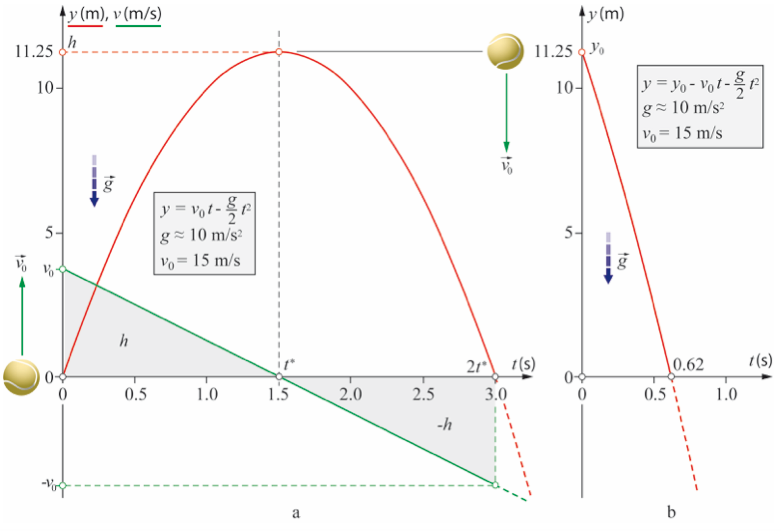
\includegraphics[width=0.9\linewidth]{images/senkrechter_wurf}
\end{minipage}
\hfill
\begin{minipage}[hbt]{0.5\linewidth}
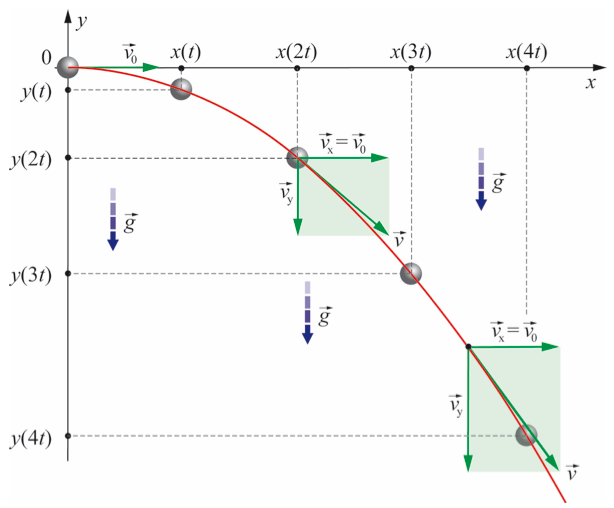
\includegraphics[width=0.9\linewidth]{images/horizontaler_wurf}
\end{minipage}


\clearpage


\subsection{Dynamik}
Die Dynamik behandelt die Kräfte als Ursache von Bewegungsabläufen. Man unterscheidet dabei die Dynamik der Translation und Rotation. (Merke: \textbf{Kraft = Gegenkraft}!)

\subsubsection{Kräfte}

\begin{itemize}
	\item Die Haft und Gleitreibung ist unabhängig von der Fläche
	\item Bei der schrägen Ebene wählt man das  Koordinaten-System mit Vorteil parallel zur Gleitebene
	\item Körper von 1kg mit $1\frac{m}{s^2}$ beschleunigen = Es wirkt eine Kraft von $1N$
	\item Beschleunigungskraft in der Schiefen Ebene: $F_B = F_H - F_G$
\end{itemize}

\begin{minipage}[h!]{0.3\linewidth}
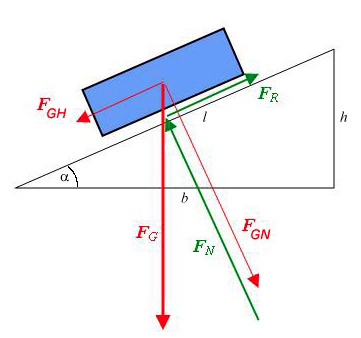
\includegraphics[width=0.9\linewidth]{images/schiefe_ebene}
\end{minipage}
\hfill
\begin{minipage}[h!]{0.2\linewidth}
	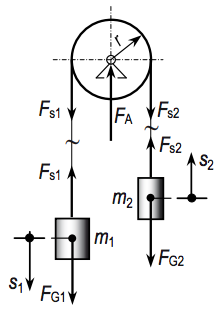
\includegraphics[width=0.9\linewidth]{images/kraefte_gleichgewicht}
\end{minipage}
\hfill
\begin{minipage}[h!]{0.4\linewidth}
\begin{align*}
m_1 \cdot a & = F_{G1} - F_{s1} \\
m_2 \cdot a & = -F_{G2} + F_{s2} \\
\Rightarrow a&=g\frac{m_1-m_2}{m_1+m_2}  \\
\Rightarrow \alpha &= \frac{a}{r} (\text{Winkelgeschwindigkeit})\\
\end{align*}
\end{minipage}

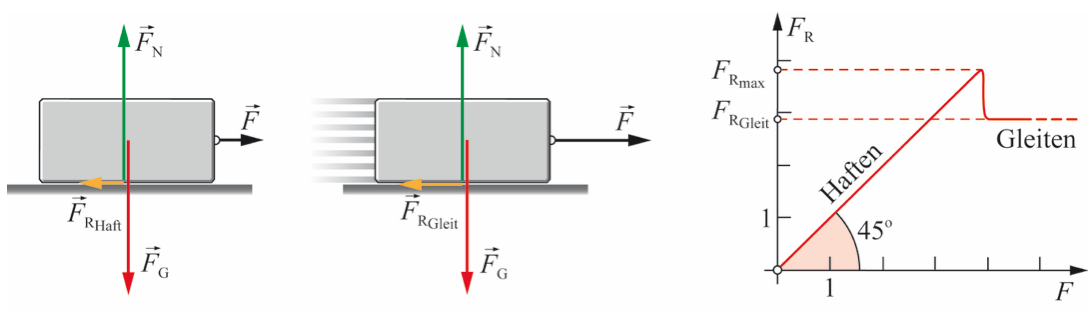
\includegraphics[width=0.9\linewidth]{images/haft_gleitkraft}


\begin{tabbing}
	\begin{tabu} to \linewidth {X l X l}
		\toprule
		Kraft & $F = m \cdot a$ & 
		Kraft in Wegrichtung & $F_s = F \cos(\alpha)$ \\
		Gewichtskraft & $F_G = mg$  &
		Federkraft (Hookesches Gesetz) & $F_F = k\cdot s$ \\
		Haftreibungskraft (max) & $F_R \leq \mu_H \cdot F_N$ &
		Gleitreibungskraft & $F_R = \mu_G \cdot F_N$ \\
		Normalkraft & $F_N = mg\cdot \cos(\alpha)$ &
		Hangabtriebskraft & $F_H = F_G \cdot \sin(\alpha)$  \\
		Zentripetalkraft & $F_r = \frac{mv^2}{r} = m\omega^2r = p\omega$ & 
		Zentrifugalkraft & $F_Z = \frac{mv^2}{r} = m\omega^2r = p\omega$ \\
		Gravitationskraft & $F_G = G \cdot \frac{m_1m_2}{r^2}$
	\end{tabu}
\end{tabbing}

\begin{tabbing}
	\begin{tabu} to \linewidth {l X l}
		Variable & Bedeutung & SI-Einheit \\
		\midrule
		$F$ & Kraft & $N = \frac{kg \cdot m}{s^2}$\\ 
		$k$ & Federkonstante & $\frac{N}{m}$ \\
		$s$ & Längenänderung & $m$ \\
		$\mu_G$ & Gleitreibungszahl &  \\
		$\mu_H$ & Haftreibungszahl &  \\
		$G$ & Gravitationskonstante = $6.67 \cdot 10^{-11}$ & $\frac{m^3}{kg s^2}$ \\
		\bottomrule
	\end{tabu}
\end{tabbing}

\paragraph{Netwonsche Axiome}

\begin{tabbing}
	\begin{tabu} to \linewidth {l l X}
		\toprule
		I Axiom & Trägheitsprinzip & $\vec{v} = const$, wenn $ \vec{F}_{res} = \vec{0}$ \\
		II Axiom & Aktionsprinzip & $\vec{F}_{res} = m\vec{a}$\\ 
		III Axiom & Wechselwirkungsprinzip & $\vec{F}_{12} = - \vec{F}_{21}$ \\
		\bottomrule
	\end{tabu}
\end{tabbing}


\subsubsection{Arbeit}

\begin{tabbing}
	\begin{tabu} to \linewidth {l X l X}
		\toprule
		Arbeit & $W = \vec F \cdot \vec s = |\vec F| |\vec s| \cos(\alpha)\,$  &
		& \\
	\end{tabu}
\end{tabbing}

\begin{tabbing}
	\begin{tabu} to \linewidth {l X l}
		Variable & Bedeutung & SI-Einheit \\
		\midrule
		$W$ & Arbeit & $Nm = J$ \\
		$s$ & Wegstrecke & $m$ \\
		\bottomrule
	\end{tabu}
\end{tabbing}

\subsubsection{Energie}
\begin{itemize}
	\item Die Energie ist eine Zustandsgrösse eines Systems, die zunimmt, wenn von aussen Arbeit am System verrichtet wird, und die abnimmt, wenn das System nach aussen Arbeit verrichtet.
	\item Energieerhaltungssatz: Die Gesamtenergie $E_{tot}$ in einem abgeschlossenen System hat einen konstanten Wert, der von Vorgängern im Symsten nicht beeinfluss wird.
	\item Die Ausdehnung einer Feder ist proportional zur Kraft
	\item \textbf{Rollen auf der schiefen Ebene}: $E_{pot} = E_{kin} + E_{rot}$
\end{itemize}
\begin{tabbing}
	\begin{tabu} to \linewidth {l X l X}
		\toprule
		Energie & $E = P \cdot t$ & Rotationsenergie & $E_{rot} = \frac{J}{2} \cdot \omega^2 $\\
		Kinetische Energie & $E_{kin} = \frac{1}{2}mv^2$ &
		Potentielle Energie & $E_{pot} = F_G \cdot h =  mgh$ \\
		Federenergie & $E_f = \frac{F \cdot s}{2} = \frac{k \cdot s^2}{2}$ &
		Federkonstante & $k = \frac{F}{s}$ \\
	\end{tabu}
\end{tabbing}

\begin{tabbing}
	\begin{tabu} to \linewidth {l X l}
		Variable & Bedeutung & SI-Einheit \\
		\midrule
		$E$ & Energie & $J = Nm = Ws = \frac{kgm^2}{s^2}$ \\
		$k$ & Federkonstante & $\frac{N}{m}$  \\
		$s$ & Strecke welche die Feder ausgedehnt wird & $m$ \\
		$J$ & Trägheitsmoment & $J = kg \cdot m^2$ \\
		\bottomrule
	\end{tabu}
\end{tabbing}

\begin{minipage}[h!]{0.4\linewidth}
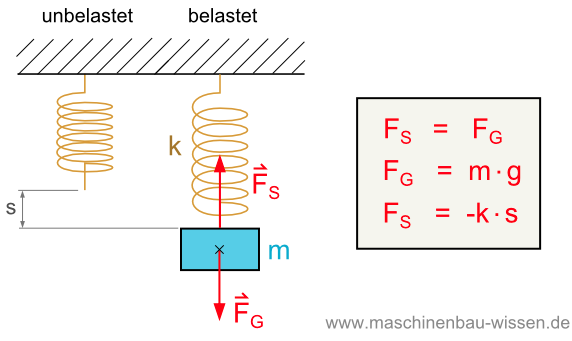
\includegraphics[width=\linewidth]{images/federenergie}
\end{minipage}
\hfill
\begin{minipage}[h!]{0.2\linewidth}
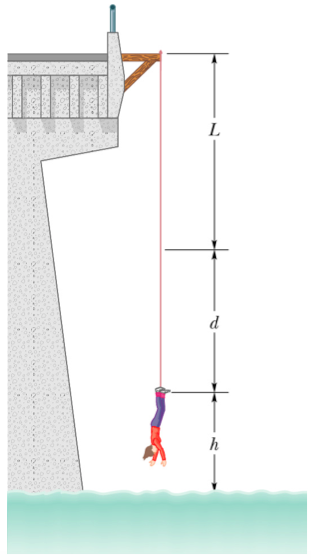
\includegraphics[width=\linewidth]{images/energie}
\end{minipage}
\hfill
\begin{minipage}[h!]{0.3\linewidth}
	\begin{align*}
	E_{pot} = E_f + E_{kin} \\
	m g (L + d) = \frac{kd^2}{2}  + \frac{m v^2}{2}  \\
	v_{Kehrpunkt} = 0 \\
	\frac{2mgL + 2mgd}{k} = d^2 \\
	d = \frac{m g}{k} \pm \frac{\sqrt{g^2 m^2 + 2 g k L m}}{k} \\
	\end{align*}
\end{minipage}

\clearpage

\subsubsection{Leistung}

\begin{tabbing}
	\begin{tabu} to \linewidth {l X l X}
		\toprule
		mittlere Leistung & $\bar{P} = \frac{W}{t}$ &
		Wirkungsgrad & $\eta = \frac{\Delta E_{ab}}{\Delta E_{zu}} = \frac{\Delta P_{ab}}{\Delta P_{zu}} < 1$ \\
		Momentanleistung & $P = F \cdot v$ & & \\
	\end{tabu}
\end{tabbing}

\begin{tabbing}
	\begin{tabu} to \linewidth {l X l}
		Variable & Bedeutung & SI-Einheit \\
		\midrule
		$P$ & Leistung & $W = \frac{J}{s} = \frac{kg \cdot m^2}{s^3}$ \\
		$E_{ab}$ & abgegebene Nutzenergie & $J$ \\
		$E_{zu}$ & aufgenommene Energie &  $J$ \\
		$W$ & verrichtete Arbeit &  $J$ \\
		$F$ & Momentankraft &  $N$ \\
		$v$ & Momentangeschwindigkeit &  $\frac{m}{s^2}$ \\
		\bottomrule
	\end{tabu}
\end{tabbing}


\subsubsection{Impuls und Stoss}
\begin{itemize}
	\item \textbf{Impulserhaltungssatz} In einem abgeschlossenen System bleibt der Impuls erhalten. Wenn nur Kräfte zwischen zwei Körpern wirken (Kraft = Gegenkraft) bleibt der Impuls erhalten. Die Bewegung des Schwerpunktes ändert sich nicht durch die Kollision.
	\item \textbf{Elastischer Stoss}  (z.B Billiardkugel) nach dem Stoss bleibt die kinetische Energie unverändert. Der Energieerhaltungssatz für die Bewegungsenergie sowie der Impulserhaltungssatz gilt. Es geht keine Energie verloren. Der Impuls vor dem Stoss = Impuls nach dem Stoss
	\begin{itemize}
		\item bewegen sich zwei Objekte aufeinander zu, ist eine Geschwindigkeit vor dem Zusammenstoss negativ.
	\end{itemize}
	\item \textbf{Unelastischer Stoss} (z.B Autounfall)
	nach dem Stoss ist die kinetische Energie kleiner. (wird in Wärme und Verformungsenergie umgewandelt) (nur der Impulserhaltungssatz gilt: $p_1 + p_2 = p_1^{'} + p_2^{'}$)
\end{itemize}


\begin{tabbing}
	\begin{tabu} to \linewidth {X l X l}
		\toprule
		Impuls & $\vec{p} = m \vec{v}$  &
		Kraftstoss & $\vec{I} = \Delta \vec{p} = \vec{F} \Delta t = m \Delta \vec{v}$ \\
		Elastischer Stoss (Obj 1) & $v_1^{'} = \frac{(m_1 - m_2) \cdot v_1 + 2 m_2 v_2}{m_1+m_2}$  &
		Elastischer Stoss (Obj 2) & $v_2^{'} = \frac{(m_2 - m_1) \cdot v_2 + 2 m_1 v_1}{m_2+m_1}$ \\
		Unelastischer Stoss & $v_1^{'} = v_2^{'} = \frac{m_1v_1 + m_2v_2}{m_1 + m_2}$ & Verformungsarbeit & $W = E_1 - E_2 = \frac{m_1m_2}{2(m_1+m_2)}(v_1-v_2)^2$ \\
	\end{tabu}
\end{tabbing}

\begin{tabbing}
	\begin{tabu} to \linewidth {l X l}
		Variable & Bedeutung & SI-Einheit \\
		\midrule
		$\vec{I}$ & Kraftstoss & $Ns = \frac{kg \cdot m}{s}$ \\
		$\vec{p}$ & Impulsänderung & $Ns = \frac{kg \cdot m}{s}$ \\
		$m$ & Masse des Körpers & $kg$ \\
		$\Delta v$ & Geschwindigkeitsänderung & $\frac{m}{s}$  \\
		$F$ & beschleunigte konstante Kraft & $N$ \\
		$\Delta t$ & Dauer der Krafteinwirkung & $s$ \\
		$v^{'}$ & Geschwindigkeit des Körpers nach dem Stoss & $\frac{m}{s}$\\
		$v$ & gemeinsame Geschwindigkeit beider Körper nach dem Stoss (unelastisch) & $\frac{m}{s}$ \\
		$W$ & Verformungsarbeit & $J$\\
		$E_1$ & Summe der Bewegungsenergie beider Körper vor dem Stoss & $J$\\
		$E_2$ & Summe der Bewegungsenergie beider Körper nach dem Stoss & $J$\\
		\bottomrule
	\end{tabu}
\end{tabbing}


\subsubsection{Dynamik der Drehbewegung}
\begin{itemize}
	\item Zentripetalkraft (Ursache für Zentralbewegung) und Zentrifugalkraft (Fliehkraft) sind gleich gross, aber entgegengerichtet.
	\item Trägheitsmoment: Bei einem drehbaren Körper ist das Verhältnis von wirkendem Drehmoment zur erzielten Winkelbeschleunigung eine konstante Grösse, dem Trägheitsmoment.
\end{itemize}
\begin{tabbing}
	\begin{tabu} to \linewidth {X l X l}
		\toprule
		Trägheitsmoment & $J = r^2\Delta m$ &
		Trägheitsmoment & $J = \sum_{i=1}^{n}r_i^2 \Delta m_i$ \\
		Zentripetalkraft & $F_r = F_z = \frac{mv^2}{r} = m\omega^2r = p\omega$ & 
		Zentripetalbeschl & $a_r = a_z = r \omega^2 = \frac{v^2}{r}$ \\
		Rotationsleistung & $P = M \omega$ &
		Rotationenergie & $E_{rot} = \frac{J\omega^2}{2}$\\
		Drehmoment & $M = J\alpha$ &
		Rotationsarbeit & $W = M\varphi$ \\
		Drehimpuls & $L = J \omega = M \cdot t = r\cdot p$ & 
		Drehimpuls einer Punktmasse & $\Delta M = \frac{\Delta L}{\Delta t}$ \\
	\end{tabu}
\end{tabbing}

\begin{tabbing}
	\begin{tabu} to \linewidth {l X l}
		Variable & Bedeutung & SI-Einheit \\
		\midrule
		$J$ & Trägheitsmoment & $J = kg \cdot m^2$ \\ 
		$m$ & Masse eines dünnen Kreisringes (Umfang) & $kg$ \\ 
		$r$ & einheitlicher Abstand aller Massenelemente von der Drehachse & $m$ \\ 
		$m_i$ & Massenelement & $kg$\\ 
		$P$ & Leistung & $W$ \\ 
		$p$ & Impuls des Körpers & $N \cdot s$ \\
		$M$ & Drehmoment, das die Drehung verursacht & $N \cdot m$ \\ 
		$\omega$ & Winkelgeschwindigkeit des Körpers & $\frac{rad}{s} = \frac{1}{s}$ \\ 
		$L$ & Drehimpuls des rotierenden Körpers & $\frac{kg \cdot m^2}{s} = N \cdot m \cdot s$  \\ 
		$\alpha$ & Winkelbeschleunigung & $\frac{rad}{s^2} = \frac{1}{s^2}$ \\
		\bottomrule
	\end{tabu}
\end{tabbing}



\begin{minipage}[h!]{0.5\linewidth}
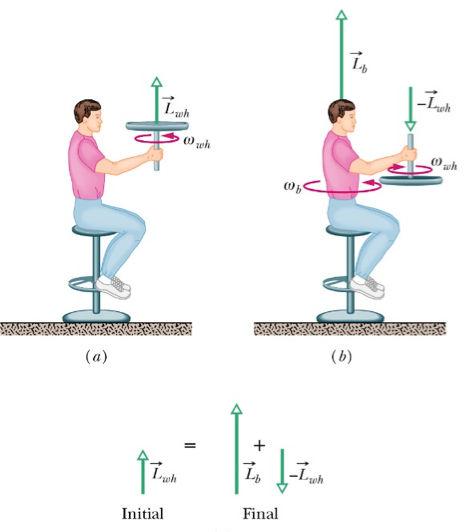
\includegraphics[width=0.8\linewidth]{images/drehimpuls}
\end{minipage}
\hfill
\begin{minipage}[h!]{0.5\linewidth}
	\begin{align*}
		L_b &= J_b \omega_b \\
		L_{wh} &= J_{wh} \omega_{wh} \\
		L_{wh} &= L_b - L_{wh} \\
		J_{wh} \omega_{wh} &= J_b \omega_b - J_{wg} \omega_{wg} \\
		\omega_b &= \frac{2J_{wh}}{J_b} \omega_{wg} \\
	\end{align*}
\end{minipage}


\clearpage


\subsection{Hydrostatik}
\begin{itemize}
	\item Druck ist Kraft pro Fläche
	\item \textbf{Das Gesetz von Pascal}: Der Druck ist eine skalare Grösse und auf jede Fläche gleich.
	\item \textbf{Hydraulische Presse}: Der Druck ist überall gleich. Die Kraft auf den Kolben ist proportional zur Fläche.
	\item \textbf{Hydrostatischer Druck}: Der Druck nimmt mit der Wassertiefe zu ($\approx$ 1 bar pro 10m Tiefe). 
	\item \textbf{Der mittlere Luftdruck} der Atmosphäre auf Meereshöhe beträgt $101'325 Pa \approx 1 bar.$	
\end{itemize}

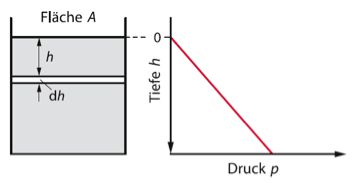
\includegraphics[width=0.4\linewidth]{images/hydrodruck}

\begin{tabbing}
	\begin{tabu} to \linewidth {l X l X}
		\toprule
		Dichte & $\rho = \frac{m}{V}$ &
		Druck (Druckkraft) & $p = \frac{F}{A}$ \\
		Auftriebskraft & $F_A = \rho_F \cdot g \cdot V_K$ &
		Schweredruck / Tiefendruck & $p = \rho g h + p_0$ \\
		Gewichtskraft & $F_G = \rho_K \cdot g \cdot V_K $ &
		Masse & $m = \rho \cdot V$ \\
	\end{tabu}
\end{tabbing}

\begin{tabbing}
	\begin{tabu} to \linewidth {l X l}
		Variable & Bedeutung & SI-Einheit \\
		\midrule
		$p$ & Druck & $1 Pa = 1\frac{N}{m^2} = 1 \frac{kg}{m\cdot s^2}$ \\ 
		$F$ & Kraft & $N$ \\
		$A$ & Fläche & $m^2$ \\
		$F_A$ & Auftriebskraft & $N$ \\
		$V_K$ & eingetauchtes Volumen (Körper), der verdrängten Flüssigkeit & $m^3$ \\
		$\rho$ & Dichte des Körpers & $\frac{kg}{m^3}$ \\
		$m$ & Masse der verdrängten Flüssigkeit & $kg$ \\
		$g$ & Fallbeschleunigung & $\frac{m}{s^2}$\\
		\bottomrule
	\end{tabu}
\end{tabbing}

\begin{minipage}[h!]{0.4\linewidth}
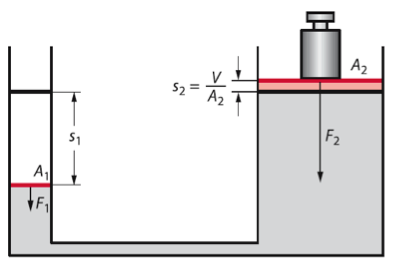
\includegraphics[width=0.8\linewidth]{images/druck}
\end{minipage}
\hfill
\begin{minipage}[h!]{0.6\linewidth}
	\textbf{Hydrostatische Presse}
	\begin{align*}
	F_1 &=p A_1 \\
	F_2 &=p A_2 \\
	\frac{F_1}{A_1} &= \frac{F_2}{A_2} \Rightarrow
	F2 = \frac{A_2}{A_1} F_1 \\
	\end{align*}
\end{minipage}

\begin{minipage}[h!]{0.4\linewidth}
	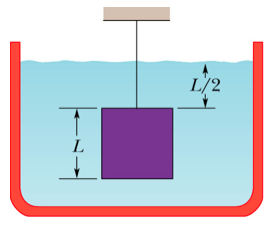
\includegraphics[width=0.8\linewidth]{images/statischer_auftrieb}
\end{minipage}
\hfill
\begin{minipage}[h!]{0.6\linewidth}
	Die Druckverteilung auf einen Körper erzeugt Auftrieb. Die benötigte Seilkraft, um ein Gewicht zu halten, ist somit. 
	\begin{align*}
	F_s= m g - \rho_f \cdot g \cdot V_E =(\rho_k - \rho_f ) \cdot g \cdot V_E
	\end{align*}
	Wenn die Dichte des Körpers $\rho_k$ kleiner als die des Fluids $\rho_f$ (z.B Holzklotz im Wasser) wird die Kraft negativ, d.h. die Gewichtskraft ist nicht gross genug damit der Klotz untertaucht. 
\end{minipage}

\subsubsection{Strömungen}

\begin{itemize}
	\item Die Ausflussgeschwindigkeit ist so gross wie nach einem freien Fall aus der Höhe h. Der Luftdruck (1bar) ist ohne Wirkung, weil er beidseitig wirkt.
	\item Der Massenfluss einer Strömung ist erhalten. Somit gilt $\dot{m} =\rho_1 v_1 A_1 = \rho_2 v_2 A_2$
\end{itemize}

\begin{minipage}[h!]{0.7\linewidth}
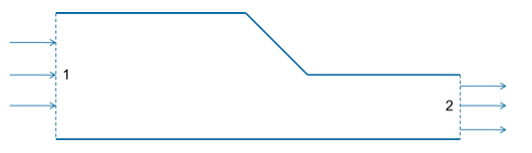
\includegraphics[width=0.7\linewidth]{images/strom_massenerhaltung}
\end{minipage}
\hfill
\begin{minipage}[h!]{0.3\linewidth}
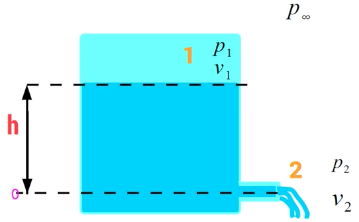
\includegraphics[width=0.9\linewidth]{images/torricelli}
\end{minipage}


\begin{tabbing}
	\begin{tabu} to \linewidth {X l X l}
		\toprule
		Ausflussgeschwindigkeit & $v_2 = \sqrt{2gh}$ &
		Kontinuitätsgleichung & $A_1v_1 = A_2v_2$ \\
		Volumenstrom & $\dot{V} = Av = \frac{V}{t} = \frac{\pi \cdot   r^4}{8  \cdot  \eta}\frac{\Delta p}{l}$ & 
		Druckdifferenz & $\Delta p = \rho \cdot g \cdot h$ \\
	\end{tabu}
\end{tabbing}

\begin{tabbing}
	\begin{tabu} to \linewidth {l X l}
		Variable & Bedeutung & SI-Einheit \\
		\midrule
		$\dot{V}$ & Volumenstrom ($\frac{1000l}{1min} = \frac{1m^3}{60s}$)& $\frac{m^3}{s}$ \\
		$v$ & mittlere Geschwindigkeit & $\frac{m}{s}$ \\
		$r$ & Innernradius des Rohrs & $m$ \\
		$l$ & Länge des Rohrs & $m$ \\
		$\eta$ & dynamische Viskosität der strömenden Flüssigkeit & $Pa \cdot s$ \\
		$\rho$ & Dichte & $\frac{kg}{m^3}$ \\
		$\Delta p$ & Druckdifferenz zwischen Anfang und Ende des Rohres & $Pa = \frac{N}{m^2} = \frac{kg}{m\cdot s^2}$ \\
		\bottomrule
	\end{tabu}
\end{tabbing}


\subsubsection{Bernoulli-Gleichung}
\begin{itemize}
	\item Die Bernoulli Gleichung wird als grundlegende Formel der Strömungslehre bezeichnet. Sie zeigt die Zusammenhänge zwischen Strömung und Energieerhaltung.
	\item Bei der stationären Strömung viskosität­sfreier inkompressibler Fluide (Flüssigkeiten und Gase) besagt sie, dass die spezifische Energie der Fluidelemente entlang einer Stromlinie konstant ist.
	\item Die Summe aus \textbf{statischem Druck} $p$, \textbf{Schweredruck} $\rho g h$ und \textbf{dynamischem Druck} $\frac{\rho}{2}v^2$ ist an jeder Stelle einer Stromlinie konstant.
	\item \textbf{Statischer Druck} folgt aus der potentiellen Energie der unter Druck stehenden Flüssigkeit
	\item \textbf{Dynamischer Druck} folgt aus der kinetischen Energie der Strömung
	\item Der \textbf{Umgebungsdruck} ist $1.013 \cdot 10^5 \frac{N}{m^2}$ und die \textbf{Dichte von Wasser} $1000\frac{kg}{m^3} = 1 \frac{kg}{l}$
\end{itemize}

\begin{tabbing}
	\begin{tabu} to \linewidth {X l}
		\toprule
		Bernoulli-Gleichung & $p_1 + \frac{\rho}{2}v_1^2 + \rho g h_1 = p_2 + \frac{\rho}{2} v_2^2 + \rho g h_2 $ \\
		Bernoulli-Gleichung (gleiche Höhe der Strömung) & $p_1 + \frac{\rho}{2} v_1^2 = p_2 + \frac{\rho}{2} v_2^2$ \\
		Torricelli Gleichung (mit Druckunterschied) & $v_2 = \sqrt{2gh + \frac{p1-p2}{\rho}}$ \\
	\end{tabu}
\end{tabbing}

\begin{tabbing}
	\begin{tabu} to \linewidth {l X l}
		Variable & Bedeutung & SI-Einheit \\
		\midrule
		$p_{1}$ & Statischer Druck an der Stelle 1 & $\frac{N}{m^2} / bar$ \\
		\bottomrule
	\end{tabu}
\end{tabbing}

\begin{minipage}[h!]{0.4\linewidth}
	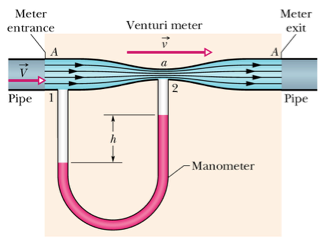
\includegraphics[width=\linewidth]{images/bernoulli}
\end{minipage}
\hfill
\begin{minipage}[h!]{0.6\linewidth}
	\begin{align*}
	V = \sqrt{\frac{2a^2 \Delta p}{\rho(A^2-a^2 )}} = \sqrt{\frac{2a^2 \rho_w gh}{\rho(A^2-a^2 )}} \\
	v_1 = \sqrt{\frac{2 \Delta p}{\omega [ (\frac{A_1}{A_2})^2 - 1 ]}}
	\end{align*}
\end{minipage}

\subsubsection{Laminare und Turbulente Strömung}
\begin{itemize}
	\item Die dimensionslose Reynolds-Zahl entscheidet, ob eine Strömung Laminar oder Viskos ist. Eine Rohrströmung ist laminar für Re<2400.
\end{itemize}

\begin{tabbing}
	\begin{tabu} to \linewidth {l X l X}
		\toprule
		Rohrreibungszahl & $\lambda = \frac{D}{\rho \cdot v^2} \frac{2dp}{dx} $  &
		Reynoldszahl & $Re = \frac{\rho \cdot v \cdot d}{\eta}$ \\
		Reibungszahl (laminar) & $\lambda_l = \frac{64}{Re}$ &
		Reibungszahl (turbulent) & $\lambda_t = \frac{0.3164}{Re^{1/4}}$ \\
		Innere Reibungskraft & $F_R = \frac{\eta A v}{d}$ &
		Druckabfall im Rohr & $\Delta p = \lambda \frac{\rho v^2}{2} \frac{l}{D}$ \\
	\end{tabu}
\end{tabbing}

\begin{tabbing}
	\begin{tabu} to \linewidth {l X l}
		Variable & Bedeutung & SI-Einheit \\
		\midrule
		$D$ & Rohrdurchmesser & $m$ \\
		$v$ & mittlere Strömungsgeschwindigkeit & $\frac{m}{s}$  \\
		$\rho$ & Dichte & $\frac{kg}{m^3}$ \\
		$d$ & charakteristische Länge  & $m$ \\
		$\eta$ & dynamische Viskosität der strömenden Flüssigkeit & $Pa \cdot s$ \\
		$A$ & Berührungsfläche & \\
		\bottomrule
	\end{tabu}
\end{tabbing}

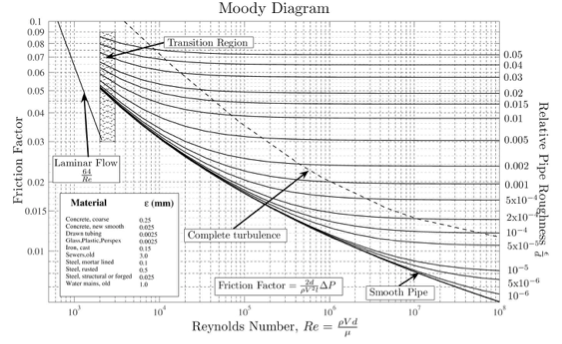
\includegraphics[width=0.8\linewidth]{images/moody_diagram}

\vfill\null
\columnbreak


\subsubsection{Strömungswiderstand}
\begin{itemize}
	\item $C_w$ ist eine dimensionslose Zahl, welche die aerodynamischen Eigenschaften des Körpers beschreibt. (z.B Auto, Kugel, Quader, Tropfen)
	\item Der Widerstandsbeiwert und der Auftriebsbeiwert eines Tragflügels sind von der Form des Flügels und von dem Anstellwinkel $\alpha$ abhängig. 
	\item Der Gleitwinkel $\phi$ gibt an, wie schnell das Flugzeug im Gleitflug an Höhe verliert.
\end{itemize}

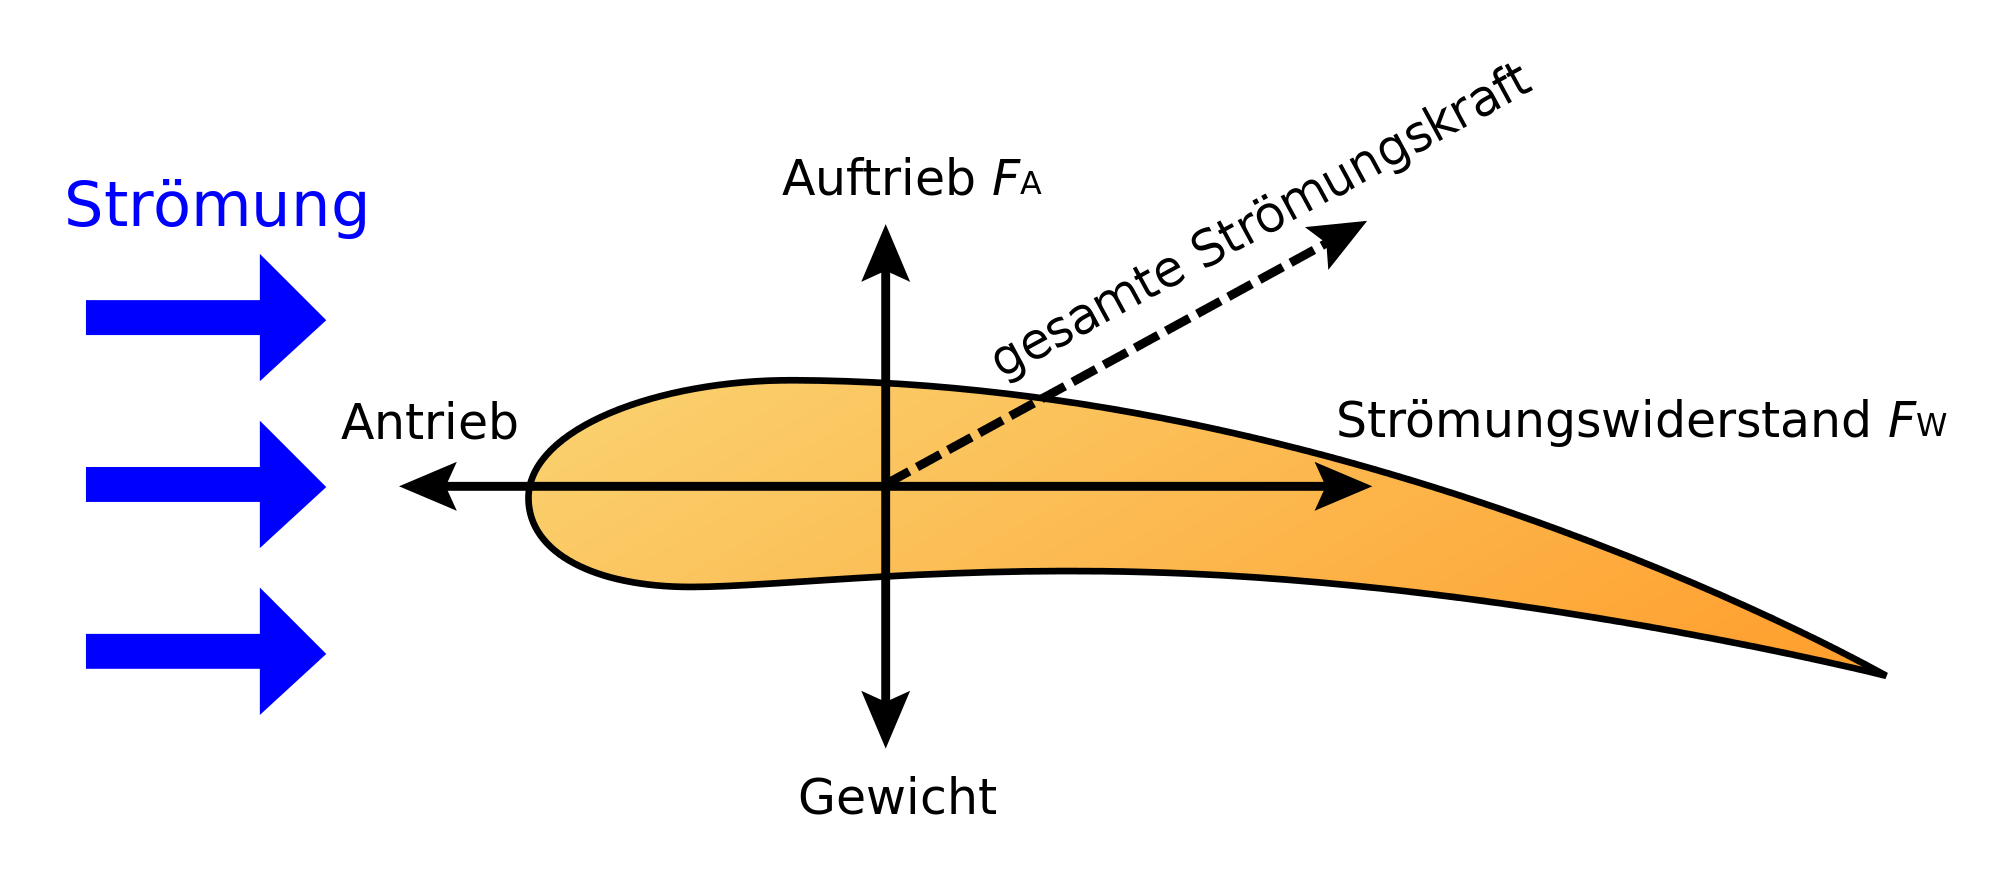
\includegraphics[width=0.6\linewidth]{images/dynamischer_auftrieb}

\begin{tabbing}
	\begin{tabu} to \linewidth {l X l X}
		\toprule
		Strömungswiderstand & $F_W = c_W  \frac{\rho}{2} v^2 A$ &
		Strömungsleistung & $P = c_W A \frac{\rho}{2}v^3$ \\
		Dynamischer Auftrieb & $F_{A} = c_{A} \frac{\rho}{2} v^2 A$ & 
		Gleitwinkel & $\tan(\phi) = \frac{c_W}{c_A}$ \\
	\end{tabu}
\end{tabbing}

\begin{tabbing}
	\begin{tabu} to \linewidth {l X l}
		Variable & Bedeutung & SI-Einheit \\
		\midrule
		$F_W$ & Strömungswiderstand & $N$\\
		$c_W$ & Widerstandsbeiwert & dimensionslos \\
		$A$ & grösster Köperquerschnitt senkrecht zur Strömung & $m$\\
		$\rho$ & Dichte & $\frac{kg}{m^3}$ \\
		$v$ & Relativgeschwindigkeit & $\frac{m}{s}$ \\	
		$\phi$ & Gleitwinkel & \\	
		\bottomrule
	\end{tabu}
\end{tabbing}

\clearpage


\section{Thermodynamik}
\begin{itemize}
	\item Die spezifische Wärmekapazität eines Stoffes gibt an, wieviel Energie zugeführt werden muss, um die Temperatur von 1 kg des Stoffes um $1^\circ \text{C}$ zu erhöhen.
	\item Die Temperatur ist ein Maß für die Bewegungsenergie der sich ungeordnet bewegenden Atome eines Systems.
	\item Wärme ist die Energie, die zwischen einem System und seiner Umgebung aufgrund eines Temperaturunterschieds ausgetauscht wird.
\end{itemize}

\paragraph{Klassifizierung}

\begin{tabbing}
	\begin{tabu} to \linewidth {l X l}
		\toprule
		Bezeichnung & Systemgrenze ist offen für & Beispiel \\
		\midrule
		Offen &	Energie und Materie	& Verbrennung \\
		Geschlossen	& Energie &	Wärmepumpe \\
		Abgeschlossen &	nichts & Thermosflasche \\
		Adiabatisch & Mechanische Arbeit (aber keine Wärme)	& Schnelle Vorgänge (z.B. Kompression) \\
		\bottomrule
	\end{tabu}
\end{tabbing}


\paragraph{0. Hauptsatz} Wenn zwei Körper die gleiche Temperatur haben, befinden sie sich in einem thermischen Gleichgewicht

\paragraph{1. Hauptsatz} Die Energie eines abgeschlossenen Systems ist erhalten.
Die Innere Energie eines Systems kann durch Zufuhr von Arbeit oder durch Zufuhr von Wärme erhöht werden.

\begin{enumerate}
	\item In einem abgeschlossenen System bleibt die Gesamtenergie konstant.
	\item Energie kann nicht erzeugt, sondern nur umgewandelt und übertragen werden. 
	\item Es gibt kein Perpetuum mobile 1. Art.
\end{enumerate}

\begin{tabbing}
	\begin{tabu} to \linewidth {l X l X}
		\toprule
		1. Hauptsatz & $\Delta U = Q + W$  &
		Kompressionsarbeit & $W = -p \Delta V$  \\
	\end{tabu}
\end{tabbing}

\begin{tabbing}
	\begin{tabu} to \linewidth {l X l}
		Variable & Bedeutung & SI-Einheit \\
		\midrule
		$\Delta U$ & Änderung der inneren Energie eines Systems &  \\
		$Q$ & Energieaustausch mit der Umgebung in Form von Wärme & \\
		$W$ & Energieaustausch mit der Umgebungin Form von Arbeit & \\
		\bottomrule
	\end{tabu}
\end{tabbing}

\paragraph{2. Hauptsatz} Die Entropie eines abgeschlossenen Systems kann nie abnehmen
\begin{enumerate}
	\item Wärme fliesst von selbst nur von einem heißen System zu einem kalten System.
	\item Keine zyklisch arbeitende Einrichtung kann Wärme vollständig in mechanishce Nutzenergie umwandeln; d.h., es gibt kein Perpetuum mobile 2. Art
	\item Abgeschlossene Systeme streben einen Zustand maximaler Unordnung bzw. grösster Wahrscheinlichkeit an. (Prinzip der max. Entropie)
\end{enumerate}

\paragraph{3. Hauptsatz}
Der absolute Nullpunkt der Temperatur -273, $16^\circ C$ (das sind 0 Kelvin) ist unerreichbar.




\subsection{Temperatur}

\subsubsection{Temperaturskalen}
\begin{itemize}
	\item Die Kelvin Skala hat ihren Nullpunkt bei der tiefsten Temperatur die theoretisch möglich ist. (absoluter Nullpunkt)
\end{itemize}
\begin{tabbing}
\begin{tabu} to \linewidth {l l l X}
	\toprule
	Fixpunkt & Celcius & Kelvin & Fahrenheit \\
	\midrule
	Gefrierpunkt & $0 \circ C$ & 273.15 K &	32 F \\
	Siedepunkt & $100 \circ C$ & 373.15 K &	212 F \\
	\bottomrule
\end{tabu}
\end{tabbing}

\vfill\null
\columnbreak

\subsection{Gasgesetze}
\begin{itemize}
	\item Das \textbf{Gesetz von Boyle-Mariotte} besagt: Bei konstanter Temperatur verhalten sich die Volumen umgekehrt wie die zugehörigen absoluten Drücke (umgekehrt proportional)
	\item Das Gesetz von Gay-Lussac besagt: Bei konstantem Volumen verhalten sich die absoluten Drücke gleich wie die zugehörigen absoluten Temperaturen (proportional) $\Rightarrow$ konstantes Volumen = Isochore
\end{itemize}

\begin{tabbing}
	\begin{tabu} to \linewidth {X l X l}
		\toprule
		Zustandsgleichung des idealen Gases & $pV = nRT = Nk_BT$  &
		Spezifische Gasgleichung & $p = \rho R_s T$ \\
		Boyle-Mariotte (konst Temperatur) & $\frac{V_1}{V_2} = \frac{p_{1}}{p_{2}} \Rightarrow pV = konst.$ &
		Gay-Lussac (konst Volumen) & $\frac{p_1}{p_2} = \frac{T_1}{T_2} \Rightarrow \frac{p}{T} = konst. $ \\
		Molzahl & $n = \frac{m}{M}$ &
		Gaskostante & $N_A \cdot k_B$\\
	\end{tabu}
\end{tabbing}
\begin{tabbing}
	\begin{tabu} to \linewidth {l X l}
		Variable & Bedeutung & SI-Einheit \\
		\midrule
		$p$ & Absolutdruck & bar  \\
		$V$ & Volumen & $m^3$  \\
		$n$ & Molzahl &  \\
		$N$ & Anzahl Teilchen &  \\
		$R$ & Gaskonstante & $8.314 \frac{J}{mol \cdot K}$  \\
		$k_B$ & Bolztmannkonstante & $1.381 \cdot 10{-23} \frac{J}{K}$ \\
		$T$ & Temperatur & Kelvin \\
		\bottomrule
	\end{tabu}
\end{tabbing}

\paragraph{Beispiel Kompression von Gasen} \hfill \\

\begin{minipage}[h!]{0.5\linewidth}
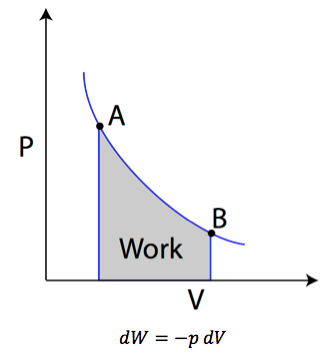
\includegraphics[width=0.8\linewidth]{images/gas_kompression}
\end{minipage}
\hfill
\begin{minipage}[h!]{0.5\linewidth}
Die Kompression eines Gases erfordert Arbeit.
\begin{align*}
dW= -p \cdot dV \\
W=- \int_{V_1}^{V_2}p \cdot dV
\end{align*}
Um das Integral berechnen zu können, brauchen wir den Druck in Abhängigkeit vom Volumen. Bei einer \textbf{isothermen} Kompression bleibt die Temperatur konstant. Aus dem idealen Gasgesetz haben wir:
\begin{align*}
p(V)=\frac{nRT}{V} \Rightarrow W = n R T \ln( \frac{V_1}{V_2})
\end{align*}
\end{minipage}

\vfill\null
\columnbreak

\subsection{Stoffmenge}
\begin{itemize}
	\item Das Gewicht von Atomen und Molekülen wird in atomic mass units ($u$) angegeben. $1u = 1.660538782(83) \cdot 10^{-27}kg$
	\item Es gilt $1g = N_A \cdot u$
	\item Die Masse eines Kohlenstoffatoms (C) ist etwa 12 u. Somit wiegt ein Mol Kohlenstoff etwa 12 g.
\end{itemize}
\begin{tabbing}
	\begin{tabu} to \linewidth {l X l X}
		\toprule
		Teilchenzahl & $N = n \cdot N_A$  &
		Stoffmenge & $n = \frac{m}{M}$  \\
		molare Masse & $M = N_A \cdot m_T$ &
		molares Volumen & $V_m = \frac{V}{n}$ \\
	\end{tabu}
\end{tabbing}
\begin{tabbing}
	\begin{tabu} to \linewidth {l X l}
		Variable & Bedeutung & SI-Einheit \\
		\midrule
		$n$ & Stoffmenge & $mol$ \\
		$N_A$ & Avogadro Konstante = 1mol & $6.02214 \cdot 10^{23} \frac{1}{mol}$  \\
		$N$ & Teilchenzahl & $mol^{-1}$ \\
		$m$ & Gasmasse & $kg$ \\
		$M$ & molare Masse & $\frac{kg}{mol}$\\
		$m_T$ & Masse eines Teilchen & \\
		\bottomrule
	\end{tabu}
\end{tabbing}


\clearpage

\subsection{Wärmeenergie}
\begin{itemize}
	\item Wenn ein Gas erwärmt wird, dehnt es sich aus. Ein Teil der zugeführten Energie wird deshalb für die Expansionsarbeit aufgewendet. Somit braucht die Erwärmung eines Gases mehr Energie.
\end{itemize}
\begin{tabbing}
	\begin{tabu} to \linewidth {l X l X}
		\toprule
		Wärmekapazität & $C = \frac{Q}{\Delta T}$  &
		Wärmekapazität (spezifisch) & $c = \frac{C}{m}$  \\
		Wärmekapazität (molar) & $C_M = \frac{C}{n}$ &
		Wärmemenge & $Q = c \dot m \Delta T $ \\
		Kondensatons, Schmelzwärme & $\dot Q_s = \dot m_D q_s$ &
		Wirkungsgrad & $\eta = \frac{\dot Q_L}{\dot Q_A} < 1$ \\
		Wärmekapazität (Gasen) & $c_p = c_v + R_i$ &
		Adiabatenexponenten & $\kappa = \frac{c_p}{c_v}$ \\
	\end{tabu}
\end{tabbing}


\begin{tabbing}
	\begin{tabu} to \linewidth {l X l}
		Variable & Bedeutung & SI-Einheit \\
		\midrule
		$Q$ & Wärmemenge & $kJ$ \\
		$C$ & Wärmekapazität &  $\frac{J}{K}$\\
		$C_m$ & molare Wärmekapazität & \\
		$c$ & spezifische Wärmekapazität & \\
		$c_p$ & spezifische Wärmekapazität bei konstantem Druck & \\
		$c_v$ & spezifische Wärmekapazität bei konstantem Volumen & \\
		$R_i$ & spezielle Gaskonstante & \\
		$n$ & Stoffmenge & \\
		$\Delta Q$ & Verhältnis der zugeführten Wärme &  \\
		$\Delta T$ & damit bewirkte Temperaturänderung &  \\
		$m$ & Masse & \\
		$\dot m_D$ & produzierte Dampf Masse & \\
		$\dot q_s$ & Verdampfungswärme / Schmelzwärme & $\frac{kJ}{kg}$\\
		$\dot Q_L$ & Wärmeleistung & $\frac{kJ}{s} = kW$\\
		$\dot Q_A$ & Wärmebelastung & $\frac{kJ}{s} = kW$\\
		\bottomrule
	\end{tabu}
\end{tabbing}

\paragraph{Äquipartitionstheorem}
\begin{itemize}
	\item Die Wärmekapazität ist von der Anzahl Freiheitsgrade abhängig. In der klassischen Physik gilt das Äquipartionstheorem
\end{itemize}
\begin{tabbing}
	\begin{tabu} to \linewidth {l X l X}
		\toprule
		Wärmekapazität & $C = \frac{f}{2}Nk_B = \frac{f}{2}nR$  & 
		& \\
	\end{tabu}
\end{tabbing}

\begin{tabbing}
	\begin{tabu} to \linewidth {l X l}
		Variable & Bedeutung & SI-Einheit \\
		\midrule
		$f$ & Anzahl Freiheitgrade bei Molekülen ($x,y,z = 3$) &  \\
		$f$ & Anzahl Freiheitgrade kristalliner Festkörper ($6$) &  \\
		$N$ & Anzahl Teilchen (Atome oder Moleküle) & \\
		\bottomrule
	\end{tabu}
\end{tabbing}

\subsubsection{Wärmeübertragung}
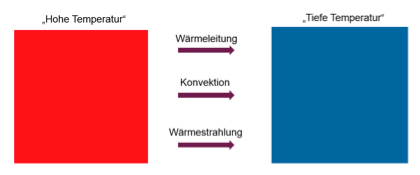
\includegraphics[width=0.5\linewidth]{images/waermetausch}

\begin{itemize}
	\item Durch direkten Kontakt: Wärmeleitung (Beispiel: Hand – kaltes Metall)
	\item Durch Strahlung: Wärmestrahlung (Beispiel: Sonne, Lebewesen)
	\item Durch Transport von Materie: Konvektion (Beispiel: Thermik)
\end{itemize}

\begin{tabbing}
	\begin{tabu} to \linewidth {l X l X}
		\toprule
		Wärmestrahlung & $\dot{Q} = \varepsilon \sigma A T ^4$  &
		 &  \\
	\end{tabu}
\end{tabbing}

\begin{tabbing}
	\begin{tabu} to \linewidth {l X l}
		Variable & Bedeutung & SI-Einheit \\
		\midrule
		$\varepsilon$ & Emissionsgrad (0 (perfekter Spiegel)-1 (Schwarzer Körper) &  \\
		$\sigma$ &  Stefan-Boltzmann-Konstante &  \\
		$A$ & Oberfläche des abstrahlenden Körpers &  \\
		$T$ & absolute Temperatur des abstrahlenden Körpers &  \\
		\bottomrule
	\end{tabu}
\end{tabbing}


\subsection{Aggregatszustände}
\begin{itemize}
	\item Die meisten Substanzen kommen in unterschiedlichen Aggregatszuständen (Phasen) vor: Fest, Flüssig und Gas. Mit den Phasenübergängen ist eine latente Wärme verbunden
\end{itemize}

\begin{minipage}[h!]{0.5\linewidth}
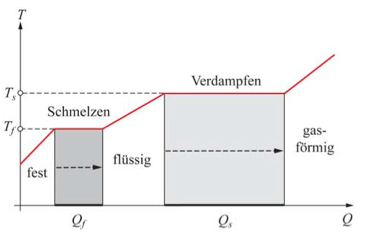
\includegraphics[width=0.8\linewidth]{images/aggregatszustaende}
\end{minipage}
\hfill
\begin{minipage}[h!]{0.5\linewidth}
\paragraph{Beispiel: Wasser}
\begin{align*}
\text{Wärmekapazität} &= C_v=4.187 \frac{kJ}{kg}kJ \\
\text{Schmelzwärme} &= Q_f = 334\frac{kJ}{kg} \\
\text{Verdampfungswärme} &= Q_s=2256\frac{kJ}{kg} \\
\end{align*}
\end{minipage}

\subsubsection{Luftfeuchtigkeit}
\begin{itemize}
	\item Der Dampfdruck von Wasser ist eine eindeutige Funktion der Temperature $p_S (T)$
	\item Der Dampfdruck entscheidet, wann Wasser kocht und definiert den Sättigungsdruck für Wasserdampf. Somit kann auch der Taupunkt berechnet werden
\end{itemize}

\begin{tabbing}
	\begin{tabu} to \linewidth {l X l X}
		\toprule
		Taupunkt & $f_r  p_s (T) = p_s (T_t)$  &
		&  \\
	\end{tabu}
\end{tabbing}

\begin{tabbing}
	\begin{tabu} to \linewidth {l X l}
		Variable & Bedeutung & SI-Einheit \\
		\midrule
		$f_r$ & relative Luftfeuchtigkeit &  \\
		$T_t$ & Temperatur des Taupunktes &  \\
		\bottomrule
	\end{tabu}
\end{tabbing}

\clearpage

\subsection{Zustandsänderung des idealen Gases}
\begin{itemize}
	\item Der 1. Hauptsatz der Wärmelehre gilt.
	\item Die innere Energie eines idealen Gases ist nur von der Temperaturänderungen abhängig
\end{itemize}

\begin{tabbing}
	\begin{tabu} to \linewidth {X l X l}
		\toprule
		Änderung der inneren Energie & $\Delta U = Q + W$  &
		Innere Energie des idealen Gases & $U = c_VmT$  \\
	\end{tabu}
\end{tabbing}

\begin{tabbing}
	\begin{tabu} to \linewidth {X l l l}
		\toprule
		Zustandsänderung & Wärmeenergie & Arbeit & Änderung der inneren Energie \\
		\midrule 
		Isochor & $\Delta Q = \Delta U$ & $\Delta W = 0$ & $\Delta U = c_V m \Delta T$ \\ 
		Isobar & $\Delta U = c_P m (T_2 - T_1)$ & $W = -p (V_2 - V_1)$ & $\Delta U = c_V m \Delta T$  \\
		Isotherm & $Q = -W$ & $ W = nRT \ln(\frac{V1}{V2}) $ & $\Delta U = 0$ \\
		Adiabatisch \hfill ($p V^\kappa = const$) & $Q = 0$ & $W = \Delta U$ & $\Delta U = c_V m \Delta T$ \\ 
	\end{tabu}
\end{tabbing}

\begin{tabbing}
	\begin{tabu} to \linewidth {l X l}
		Variable & Bedeutung & SI-Einheit \\
		\midrule
		$Q$ & mit der Umgebung ausgetauschte Wärmeenergie &  \\
		$W$ & am System verrichtete mechanische Arbeit &  \\
		$c_p$ & spezifische Wärmekapazität bei konstantem Druck &  \\
		$m$ & Masse des Gases &  \\
		\bottomrule
	\end{tabu}
\end{tabbing}

\subsubsection{Thermischer Wirkungsgrad des Carnot-Prozesses}
\begin{itemize}
	\item Wir betrachten einen Maschine, welche Wärme von einem heissen Reservoir transportiert und gleichzeitig Arbeit leistet (Dampfmaschine, Stirling-Motor)
\end{itemize}
\begin{tabbing}
	\begin{tabu} to \linewidth {X l X l}
		\toprule
		Carnot Wirkungsgrad & $\eta_C = \frac{T_1 - T_2}{T_1} = 1 - \frac{T_2}{T_1}$  & 
		Wirkungsgrad & $\eta = \frac{Q_{zu} + Q_{ab}}{Q_{zu}} = 1- \frac{Q_{ab}}{Q_{zu}} \leq 1 - \frac{T_{ab}}{T_{zu}}$  \\
	\end{tabu}
\end{tabbing}

\begin{tabbing}
	\begin{tabu} to \linewidth {l X l}
		Variable & Bedeutung & SI-Einheit \\
		\midrule
		$S$ &Entropie & $\frac{J}{K}$ \\
		\bottomrule
	\end{tabu}
\end{tabbing}

\begin{minipage}[h!]{0.5\linewidth}
	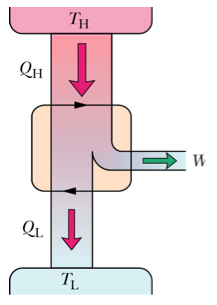
\includegraphics[width=0.4\linewidth]{images/carnot_machine}
\end{minipage}
\hfill
\begin{minipage}[h!]{0.5\linewidth}
Wir wollen einen Dampfmaschine mit einer Temperatur von $T_H=120C^\circ$ betreiben. Das Kühlwasser hat eine Temperatur von $T_L=10C^\circ$. Der maximale Wirkungsgrad ist dann
\[
	\eta = 1 - \frac{283K}{393 K} \approx 0.25 
\]
\end{minipage}

\vfill\null
\columnbreak

\subsubsection{Entropie}
\begin{tabbing}
	\begin{tabu} to \linewidth {l X l X}
		\toprule
		Entropieänderung & $dS = \frac{dQ_{rev}}{T}$  &  &  \\
	\end{tabu}
\end{tabbing}

\begin{tabbing}
	\begin{tabu} to \linewidth {l X l}
		Variable & Bedeutung & SI-Einheit \\
		\midrule
		$S$ &Entropie & $\frac{J}{K}$ \\
		\bottomrule
	\end{tabu}
\end{tabbing}

\begin{minipage}[h!]{0.3\linewidth}
	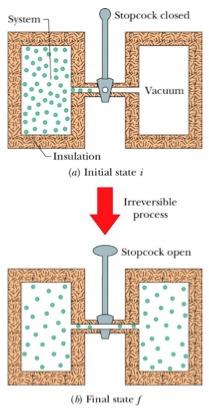
\includegraphics[width=0.8\linewidth]{images/entropie}
\end{minipage}
\hfill
\begin{minipage}[h!]{0.6\linewidth}
Bei diesem Experiment ändert sich die Energie des Systems nicht. Die Entropie nimmt aber zu. Deshalb ist das Experiment irreversibel: Das Gas wird nicht von sich aus zurückfliessen. Dies ist ein statistischer Effekt
\end{minipage}


\clearpage

\subsection{Wärmetransport}

\begin{minipage}[h!]{0.5\linewidth}
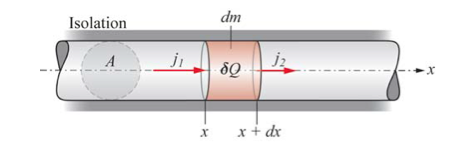
\includegraphics[width=\linewidth]{images/waermestromdichte}
\end{minipage}
\hfill
\begin{minipage}[h!]{0.5\linewidth}

\end{minipage}

\begin{tabbing}
	\begin{tabu} to \linewidth {l X l X}
		\toprule
		Wärmestromdichte & $j_q=- \lambda \frac{dT}{dx}$ &
		Wärmeübergang (Konvektion) & $j_q=\alpha (T-T_w)$ \\
		Wärmedurchgang & $Q = k A \Delta T$ &
		Wärmedurchgangskoeffizient & $ \frac{1}{k} = \frac{1}{\alpha_1} + \frac{1}{\alpha_2} + \frac{l}{\lambda} $ \\
	\end{tabu}
\end{tabbing}

\begin{tabbing}
	\begin{tabu} to \linewidth {l X l}
		Variable & Bedeutung & SI-Einheit \\
		\midrule
		$Q$ & durch die ebene Wand übertragenen Wärmemenge & $J$ \\
		$k$ & Wärmeduchgangskoeffizient & $\frac{W}{m^2K}$\\
		$A$ & Grösse der Durchgangsfläche & $m^2$\\
		$l$ & Wanddicke & $m$ \\
		$t$ & Zeit des Durchgangs & $s$ \\
		$\Delta T$ & Temperaturdifferenz zwischen den Medien vor und hinter der Wand & \\
		$j_q$ & Wärmestromdichte & $\frac{W}{m^2}$ \\
		$\lambda$ & Wärmeleitfähigkeit & $\frac{W}{mK}$ \\
		$\alpha$ & Wärmeübergangskoeffizient & $\frac{W}{m^2K}$ \\
		\bottomrule
	\end{tabu}
\end{tabbing}

\paragraph{Beispiel: Wärmeverlust Haus}
Die benötigte Heizleistung eines Hauses ist gegeben durch die Summe der Wärmflüsse durch alle Flächen ($Q_w$) plus den Luftaustausch mit der Aussenluft. ($Q_L$)
\begin{align*}
\dot{Q} &= \dot{Q_w}  + \dot{Q_L} \\
		&= (\sum_q(A_q k_q+\rho c_p \dot{V}) \Delta T
\end{align*}


\paragraph{Beispiel: Wärmedurchgang durch eine ebene Wand} \hfill \\
\begin{minipage}[h!]{0.5\linewidth}
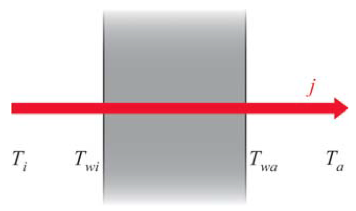
\includegraphics[width=0.8\linewidth]{images/waermedurchgang}
\end{minipage}
\hfill
\begin{minipage}[h!]{0.5\linewidth}
	\begin{align*}
	\text{Übergangsschicht innen:  } j &= \alpha_i (T_i - T_{wi}) \\
	\text{Wärmeleitung in der Wand:  } j &= \frac{\lambda}{d}(T_{wi} - T_{wa}) \\
	\text{Übergangsschicht aussen:  }  j &= \alpha_i (T_{wa} - T_{a})  \\
	\end{align*}
\end{minipage}


\vfill\null
\columnbreak

\subsection{Temperaturstrahlung}
\begin{itemize}
	\item Ein Körper mit den (nicht realisierbaren) Eigenschaften $\varrho = 0, \tau = 0, \alpha = 1$ heisst schwarzer Körper
	\item Absorption $\alpha$ = Emission $\varepsilon$
	\item Das Emissionsverhältnis und Absorptionsverhältnis sind beide im Bereich [0,1]
\end{itemize}

\begin{tabbing}
	\begin{tabu} to \linewidth {X l X l}
		\toprule
		Stefan-Boltzmann'sche Gesetz & $P = \sigma \varepsilon AT^4$ &
		Emissionsvermögen (schwarzer Körper) & $P = \sigma T^4$ \\
		Kirchhoff'sche Strahlungsgesetz & $\varepsilon(\lambda, T) = \alpha(\lambda, T)$ & & \\
	\end{tabu}
\end{tabbing}

\begin{tabbing}
	\begin{tabu} to \linewidth {l X l}
		Variable & Bedeutung & SI-Einheit \\
		\midrule
		$P$ & Strahlungsleistung & \\
		$\varepsilon$ & Emissionsgrad & \\
		$A$ & strahlende Oberfläche des Körpers & \\
		$\sigma$ & Stefan-Boltzmann-Konstante, Strahlungskonstante & $5.670373 \cdot 10^{-8} \frac{W}{m^2 K^4}$ \\
		\bottomrule
	\end{tabu}
\end{tabbing}

\clearpage

\section{Elektrizitätslehre}
\subsection{Elektrischer Stromkreis}
\begin{tabbing}
	\begin{tabu} to \linewidth {l X l X}
		\toprule
		Stromstärke & $I = \frac{\Delta Q}{\Delta t}$ & 
		Widerstand & $R = \frac{U}{I}$ \\
		Ohmsches Gesetz & $U = R \cdot I$ & 
		Widerstand eines Drahtes & R = $\rho_{el} = \frac{l}{A}$ \\
		Elektrische Leistung & $P = UI = \frac{U^2}{R} = I^2 R$ & 
		Elektrische Arbeit & $W = UI\Delta t$ \\
		Stromkosten & $K = W \cdot T$ & \\
		Kapazität Kondensators & $C= \frac{\varepsilon A}{d} \Leftrightarrow Q = CU$ &
		El. Energie Kondensator & $E=\frac{1}{2} CU^2$\\
	\end{tabu}
\end{tabbing}


\begin{tabbing}
	\begin{tabu} to \linewidth {l X l}
		Variable & Bedeutung & SI-Einheit \\
		\midrule
		$U$ & Spannung & $V$ \\
		$R$ & Widerstand & $\Omega$ \\
		$l$ & länge des Drahtes & \\
		$\rho_{el}$ & spezifischer Widerstand & \\
		$I$ & Stromstärke & $A$ \\
		$Q$ & geflossene Ladung & $As = C \text{ (couloumb)}$ \\
		$P$ & Leistung & $W$ \\	
		$W$ & Arbeit & $Ws / kwH$ \\
		$T$ & Tarif & $\frac{Fr.}{kWh}$ \\
		$K$ & Kosten & $Fr.$ \\
		\bottomrule
	\end{tabu}s
\end{tabbing}


\end{multicols*}

\end{document}
